\documentclass{beamer}
\usepackage[utf8]{inputenc}

\usetheme{Madrid}
\usecolortheme{default}
\usepackage{amsmath,amssymb,amsfonts,amsthm}
\usepackage{mathtools}
\usepackage{txfonts}
\usepackage{tkz-euclide}
\usepackage{listings}
\usepackage{adjustbox}
\usepackage{array}
\usepackage{gensymb}
\usepackage{tabularx}
\usepackage{gvv}
\usepackage{lmodern}
\usepackage{circuitikz}
\usepackage{tikz}
\lstset{literate={·}{{$\cdot$}}1 {λ}{{$\lambda$}}1 {→}{{$\to$}}1}
\usepackage{graphicx}

\setbeamertemplate{page number in head/foot}[totalframenumber]

\usepackage{tcolorbox}
\tcbuselibrary{minted,breakable,xparse,skins}



\definecolor{bg}{gray}{0.95}
\DeclareTCBListing{mintedbox}{O{}m!O{}}{%
  breakable=true,
  listing engine=minted,
  listing only,
  minted language=#2,
  minted style=default,
  minted options={%
    linenos,
    gobble=0,
    breaklines=true,
    breakafter=,,
    fontsize=\small,
    numbersep=8pt,
    #1},
  boxsep=0pt,
  left skip=0pt,
  right skip=0pt,
  left=25pt,
  right=0pt,
  top=3pt,
  bottom=3pt,
  arc=5pt,
  leftrule=0pt,
  rightrule=0pt,
  bottomrule=2pt,
  toprule=2pt,
  colback=bg,
  colframe=orange!70,
  enhanced,
  overlay={%
    \begin{tcbclipinterior}
    \fill[orange!20!white] (frame.south west) rectangle ([xshift=20pt]frame.north west);
    \end{tcbclipinterior}},
  #3,
}
\lstset{
    language=C,
    basicstyle=\ttfamily\small,
    keywordstyle=\color{blue},
    stringstyle=\color{orange},
    commentstyle=\color{green!60!black},
    numbers=left,
    numberstyle=\tiny\color{gray},
    breaklines=true,
    showstringspaces=false,
}
%------------------------------------------------------------
%This block of code defines the information to appear in the
%Title page
\title %optional
{5.2.29}
\date{September 5,2025}
%\subtitle{A short story}

\author % (optional)
{Harsha-EE25BTECH11026}



\begin{document}


\frame{\titlepage}


\begin{frame}{Question}
Solve for the system of linear equations:
\begin{align*}
    x+3y=6\\
    2x-3y=12
\end{align*}

\end{frame}

\begin{frame}{Theoretical Solution}
According to the question,\\
The equation of lines given,
\begin{align}
    \myvec{1&&3}\vec{x}=6 \quad \myvec{2&&-3}\vec{x}=12
\end{align}
\begin{align}
    \therefore \myvec{1&&3\\2&&-3}\vec{x}=\myvec{6\\12}
\end{align}
\end{frame}

\begin{frame}{Theoretical Solution}
Forming an augmented matrix,
\begin{align}
    \augvec{2}{1}{1&3&6\\2&-3&12}
\end{align}
Upon doing row reduction,
\begin{align}
\begin{aligned}
     \augvec{2}{1}{1&3&6\\2&-3&12}
     \xleftrightarrow{\,R_2 \gets R_2- 2 \times R_1}
     \augvec{2}{1}{1&3&6\\0&-9&0}  
     \xleftrightarrow{\,R_1 \gets R_1+ \frac{1}{3} \times R_2}
     \augvec{2}{1}{1&0&6\\0&-9&0}
\end{aligned}
\end{align}
\begin{align}
    \implies \vec{x}=\myvec{6\\0}
\end{align}
\end{frame}


\begin{frame}[fragile]
    \frametitle{C Code -Finding Solution for the system of Equations}

    \begin{lstlisting}[language=C]
#include <stdio.h>

void rref_solver(double aug[2][3], double solution[2]) {
    // Normalize first row (pivot = aug[0][0])
    double pivot = aug[0][0];
    for (int j = 0; j < 3; j++) {
        aug[0][j] /= pivot;
    }
    // Eliminate below pivot
    double factor = aug[1][0];
    for (int j = 0; j < 3; j++) {
        aug[1][j] -= factor * aug[0][j];
    }



    \end{lstlisting}
\end{frame}

\begin{frame}[fragile]
    \frametitle{C Code -Finding Solution for the system of Equations}

    \begin{lstlisting}[language=C]
    // Normalize second row (pivot = aug[1][1])
    pivot = aug[1][1];
    for (int j = 0; j < 3; j++) {
        aug[1][j] /= pivot;
    }
    // Eliminate above pivot
    factor = aug[0][1];
    for (int j = 0; j < 3; j++) {
        aug[0][j] -= factor * aug[1][j];
    }
    // Extract solution
    solution[0] = aug[0][2]; // x
    solution[1] = aug[1][2]; // y
}


    \end{lstlisting}
\end{frame}

\begin{frame}[fragile]
    \frametitle{Python+C code}

    \begin{lstlisting}[language=Python]
import ctypes
import numpy as np
import matplotlib.pyplot as plt
import matplotlib as mp
mp.use("TkAgg")
# Load the shared C library
lib = ctypes.CDLL("./liblineq_solver.so")
# Define argument and return types
lib.rref_solver.argtypes = [ctypes.c_double * 6, ctypes.c_double * 2]
# Create augmented matrix for system:
aug = (ctypes.c_double * 6)(1, 3, 6,   2, -3, 12)  # Flattened 2x3
solution = (ctypes.c_double * 2)()
lib.rref_solver(aug, solution)
# Convert result to numpy vector (ensure flat)
x_sol = np.array([solution[0], solution[1]], dtype=float).flatten()
print("Solution vector from C:", x_sol)


    \end{lstlisting}
\end{frame}

\begin{frame}[fragile]
    \frametitle{Python+C code}

    \begin{lstlisting}[language=Python]
# plot
x_vals = np.linspace(-2, 10, 400)
y1 = (6 - x_vals) / 3
y2 = (12 - 2*x_vals) / -3

plt.plot(x_vals, y1, label=r"$x+3y=6$")
plt.plot(x_vals, y2, label=r"$2x-3y=12$")

plt.scatter(x_sol[0], x_sol[1], color="red", zorder=5)
plt.text(float(x_sol[0])+0.2, float(x_sol[1]), f"({x_sol[0]:.1f}, {x_sol[1]:.1f})", color="red")


    \end{lstlisting}
\end{frame}

\begin{frame}[fragile]
    \frametitle{Python+C code}

    \begin{lstlisting}[language=Python]
plt.xlabel("x")
plt.ylabel("y")
plt.title("Garphical solution of the Linear system")
plt.axhline(0, color="black", linewidth=0.8)
plt.axvline(0, color="black", linewidth=0.8)
plt.legend()
plt.grid(True)
plt.savefig("/home/user/Matrix/Matgeo_assignments/5.2.29/figs/Figure_1.png")
plt.show()
    \end{lstlisting}
\end{frame}

\begin{frame}[fragile]
    \frametitle{Python code}
    \begin{lstlisting}[language=Python]
import numpy as np
import matplotlib.pyplot as plt
import matplotlib as mp
mp.use("TkAgg")

A=np.array([[1,3],[2,-3]],dtype=float)
b=np.array([6,12], dtype=float)

x=np.linalg.solve(A,b)
print("Solution vector for the system of equations:",x)
    \end{lstlisting}   
\end{frame}

\begin{frame}[fragile]
    \frametitle{Python code}
    \begin{lstlisting}[language=Python]
# Making a plot
x_vals = np.linspace(-2, 10, 400)

# Rearranged equations to express y in terms of x
y1 = (6 - x_vals) / 3        # from x + 3y = 6
y2 = (12 - 2*x_vals) / -3    # from 2x - 3y = 12

# Plot lines
plt.plot(x_vals, y1, label=r"$x + 3y = 6$")
plt.plot(x_vals, y2, label=r"$2x - 3y = 12$")

# Mark solution
plt.scatter(x[0], x[1], color="red", zorder=5)
plt.text(x[0]+0.2, x[1], f"({x[0]:.1f}, {x[1]:.1f})", color="red")
    \end{lstlisting}
    
\end{frame}

\begin{frame}[fragile]
    \frametitle{Python code}
    \begin{lstlisting}[language=Python]
# Formatting
plt.xlabel("x")
plt.ylabel("y")
plt.title("Graphical Solution of the Linear System")
plt.axhline(0, color='black', linewidth=0.8)
plt.axvline(0, color='black', linewidth=0.8)
plt.legend()
plt.grid(True)
plt.savefig("/home/user/Matrix/Matgeo_assignments/5.2.29/figs/Figure_1")
plt.show()
    \end{lstlisting}  
\end{frame}


\begin{frame}{Plot}
    \begin{figure}[H]
    \centering
    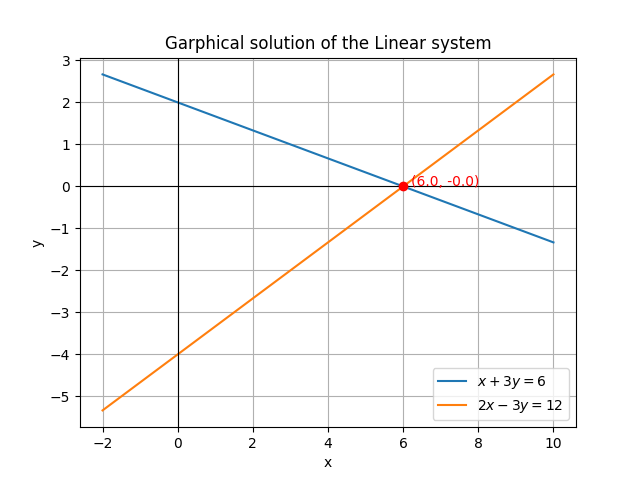
\includegraphics[width=0.6\columnwidth]{figs/Figure_1.png}
    \label{fig:1}
\end{figure}
\end{frame}

\end{document}